\documentclass[conference]{IEEEtran}
\IEEEoverridecommandlockouts
% The preceding line is only needed to identify funding in the first footnote. If that is unneeded,  please comment it out.
\usepackage{cite}
\usepackage{amsmath, amssymb, amsfonts}
\usepackage{graphicx}
\usepackage{textcomp}
\usepackage{xcolor}
\usepackage[marginal]{footmisc}
\def\BibTeX{{\rm B\kern-.05em{\sc i\kern-.025em b}\kern-.08em
    T\kern-.1667em\lower.7ex\hbox{E}\kern-.125emX}}
\begin{document}

\title{Adversarial Training for Supervised Relation Extraction}

\author{\IEEEauthorblockN{1\textsuperscript{st} Yanhua Yu}
\IEEEauthorblockA{\textit{Beijing University of }\\
\textit{Posts and Telecommunications} \\
Beijing, China \\
yuyanhua@bupt.edu.cn}
\and
\IEEEauthorblockN{2\textsuperscript{nd} Kanghao He}
\IEEEauthorblockA{\textit{Beijing University of }\\
\textit{Posts and Telecommunications} \\
Beijing, China \\
hkh@bupt.edu.cn}
\and
\IEEEauthorblockN{3\textsuperscript{rd} Jie Li}
\IEEEauthorblockA{\textit{Beijing University of }\\
\textit{Posts and Telecommunications} \\
Beijing, China \\
jli@bupt.edu.cn}
}

\maketitle

\begin{abstract}
  Most supervised methods for relation extraction(RE) need lots of time-consuming human annotation.
Distant supervision for relation extraction is an efficient method to obtain large corpora which contains thousands of instances and various relations.
However, the existing approaches rely on sophisticated pre-defined rules as well as knowledge base(e.g Freebase) for automatic annotation and thus suffer from data noise.
Various relations and noisy labeling instances make the issue harder to be solved.
To address these issues, we build a relation candidate set and then apply an adversarial training mechanism to filter out those noisy instances from the candidate set and identify informative ones.
The experiments on the extended dataset show that our candidate selection and generative adversarial network can cooperate together to obtain more accurate training data for RE and significantly outperforms several competitive baseline models. 
\end{abstract}

\begin{IEEEkeywords}
relation extraction, adversarial training, generative adversarial network
\end{IEEEkeywords}

\section{Introduction}
Relation extraction(RE), which aims to extract relations between entity pairs from the sentences containing them, is of great importance for many
natural language applications, such as information extraction, question answering and 
construction of knowledge base(KB)\cite{Fader2011IdentifyingRF, Xu2016Question, Bollacker2008FreebaseAC}.

Most prior methods for RE follow a supervised learning approach to train models on human-annotated data, such as SemEval-2010 Task 8\cite{hendrickx2009semeval} and ACE 2005\cite{Ace2005}.
These methods are limited by the amount of labeled training data, thus Mintz\cite{mintz2009distant} proposes distant supervision to automatically generate training data based on knowledge bases.
It assumes that if two entities have a relation in KBs, then all sentences mentioning these two entities express this relation.
Thus, distant supervision can generate abundant amounts of labeled data without intensive labor.
Simultaneously, it always suffers from wrong labeling problem.
For example, (Apple, founder, Steve Jobs) is a relational fact in KB, the sentence "Steve Jobs passed away the day before Apple unveiled iPhone 4s in late 2011." does not express the relation founder but will still be regarded as a training instance.
To combat the noisy training data, Riedel and Hoffmann \cite{riedel2010modeling, hoffmann2011knowledge} propose multi-instance learning, assuming only that at least one of the sentences containing
entities are expressing the relation.
Zeng and Santos attempt to incorporate multi-instance learning with neural network model \cite{zeng2015distant, zeng2016incorporating, santos2015classifying}.
Recently, attention mechanisms have been proposed to select valid instances from the auto-annotated sentence set \cite{lin2016neural, ZHOU2018240}.

Although these methods achieve significant improvement in relation extraction, there are still some severe problems for these RE methods:
(1)Most supervised datasets lack sufficient training data.
(2)Distant supervision naturally suffers from the inevitable noisy data, and the supervision is much weaker due to the multi-instance framework.

In this paper, we propose an approach which uses generative adversarial network to take advantage of the noisy data and a discovery strategy to obtain more labeled data.
Considering the weakness of distant supervision, we use supervised dataset and adopt a discovery strategy similar to distant supervision, assuming that if two entities have a relation in supervised training set, then all
instances mentioning these two entities express this relation.
Hence, we obtain a supervised dataset and a noisy dataset.
These noisy data that come from heuristic labeling are natural adversarial training samples.
We design a generative adversarial network consisting of a selector and a discriminator like Goodfellow\cite{goodfellow2014explaining}, as shown in Figure 1.

\footnote{
  \noindent
  \textbf{收稿日期}: 2020-5-31 \\
  \
}

\begin{figure*}[h]
  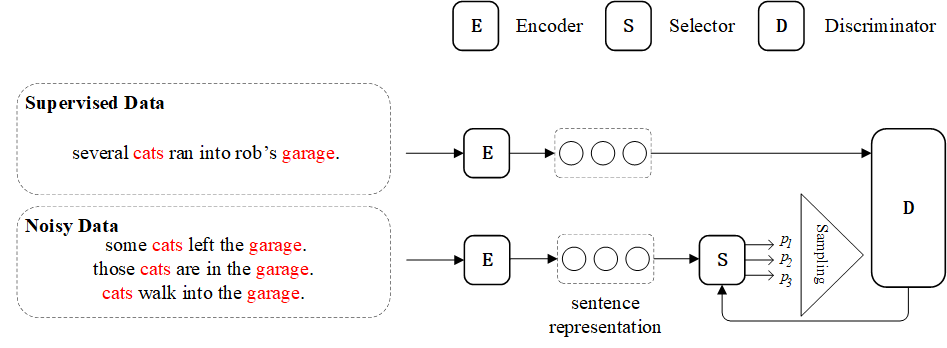
\includegraphics[height=6cm]{architecture.png}
  \caption{The overall architecture of generative adversarial network. The relation type is \textit{Entity-Destination(e1, e2)}. The sentence in Supervised Data comes from SemEval-2010 Task 8 dataset and the sentences in Noisy Data are discovered by our discovery strategy. }
  \label{Architecture}
\end{figure*}

The selector is used to select the most confusing instance from the noisy data and the discriminator is used to judge whether a instance is annotated correctly.
During the training process, the discriminator will influence the selector to select the more informative data and thus the discriminator will integrate information from supervised data and adversarial data.  
When the selector and the discriminator reach a balance, the selector can effectively select valid instances to the discriminator and the discriminator can boost resistance to noise and improve the relation extraction.
Instances from the noisy dataset selected by the selector and regarded as being labeled correctly by the discriminator will be judged as valid data and enrich the supervised dataset.
\\Our main contributions are listed as follows:
\begin{itemize}
  \item Compared with existing neural relation extraction model, we propose a novel adversarial training mechanism to make full use of all informative sentences of noisy data.
  \item The discovery strategy and the selector can cooperate to obtain more valid training data and extend the original supervised dataset.
  \item Experiments on the extension of SemEval-2010 Task 8 dataset have demonstrated that our model significantly outperforms the previous models, and the new dataset improves the performance of previous models as well.
\end{itemize}

\section{Related Work}
This paper is mainly related to neural networks and adversarial training.
Most traditional supervised RE models \cite{socher2012semantic, zeng2014relation, santos2015classifying} heavily rely on abundant amounts of annotated data, which are labor intensive and time consuming.
To address this issue, Mintz\cite{mintz2009distant} proposed a distantly supervised model for RE.
Distant supervision aligns plain text with Freebase to automatically label large-scale training data.
However, the training data generated by distant supervision inevitably accompany with the mislabeling problem.
Therefore, mainstream methods of distant supervision focus on reducing noise.

To alleviate the noise issue, Riedel\cite{riedel2010modeling} and Hoffmann\cite{hoffmann2011knowledge} proposed multi-instance learning (MIL) mechanisms for single-label and multi-label problems respectively, where instances are processed at a bag level.
But these feature-based methods depend strongly on the handcrafted features.
Most features are explicitly generated by NLP tools, which will suffer from error propagation problem.
With the development of neural networks, various neural methods have been proposed.
Zeng\cite{zeng2015distant} attempted to integrate piecewise convolution neural network(PCNN) into distant supervision.
The method assumes that at least one sentence that mentions these two entities will express their relation and select the most reliable sentence as the bag representation.
Lin\cite{lin2016neural} further proposed attention mechanism to jointly consider all sentences containing same entity pairs and distribute different weights to each sentence.
Attention-based neural relation extraction (NRE) model has become a foundation for some recent works\cite{liu2017soft, ZHOU2018240}.
Yuan\cite{yuan2018crossrelation} conduct MIL with a cross-relation cross-bag selective attention in order to reduce the impact of noisy data.
Ye\cite{ye-ling-2019-distant} adopted both intra-bag and inter-bag attention to deal with the noisy training data.
Apart from that, some efforts have been made to improve the performance of RE with external knowledge, entity description, and reinforcement learning\cite{han2018neural, ji2017, feng2018reinforcement}.
Nevertheless, due to the restriction of knowledge bases as well as the lack of external information, those methods still suffer from the noise at sentence-level and bag-level respectively.

Adversarial training has been widely exploited in NLP applications recently to resist noise including text classification and relation extraction\cite{miyato2016adversarial, wu2017adversarial, qin2018dsgan}.
For example, Wu\cite{wu2017adversarial} generated adversarial instances by adding simple noise perturbation to embeddings.
Qin\cite{qin2018dsgan} adopted adversarial training to denoise data and neglect to discover more training instances from raw data.

Different from the existing methods, our work regard the real-world data as adversarial samples rather than add pseudo noisy perturbations.
Furthermore, we propose a discovery strategy similar to distant supervision and train a selector(the generator) so that our model not only resist the noisy data but also discover valid labeled data to extend datasets.
Our discovery strategy can obtain specific relation type to deal with the imbalanced dataset.

\section{Methodology}
In this section, we present the overall framework of our model for supervised relation extraction with discovery strategy.
After that, we present each module in details.
\subsection{Preliminaries}
The architecture of the generative adversarial network is illustrated in Figure 1, which has three main modules including sentence encoder, selector and discriminator.

The sentence encoder is applied to transform sentences into low-dimensional vectors.
Given a sentence $s$ and two target entities, a piecewise convolution neural network(PCNN)\cite{zeng2015distant} is used to derive the sentence representation $\mathbf{x}$.Details of the sentence encoder are shown in Section ~\ref{sect:encoder}.

After that, we introduce an adversarial learning pipeline to train a selector which can select the valid instances from the noisy dataset ND under the guidance of the discriminator.
The discriminator is responsible for judging whether the given instance expresses its relation. 
The adversarial training strategy is the core of our method.
We will give its details in Section ~\ref{sect:ad}.

Our discovery strategy is based on a heuristic assumption that if a given pair of entities have a relation in supervised dataset SD, all other sentences mentioning these two entities express this relation.
If an instance does not contain a pair of entities shown in SD, it will be labeled with \textit{NA}.
It is effective to obtain abundant amounts of adversarial noisy data ND.
The details of automatically labeling ND and utilizing selector to extend SD will be introduced in Section ~\ref{sect:extend}. 
\subsection{Sentence Encoder} 
\label{sect:encoder} 
\subsubsection*{Input representation}

\textbf{Word Embeddings.}Given a sentence $x$ consisting of $m$ words $x = \left \{w_{1}, w_{2}, ..., w_{m}  \right \}$, each word $w_{i}$ is mapped into a $d_{w}$-dimensional word embedding $\mathbf{w}_i$, where $\mathbf{w}_i$ is the pre-trained word vector of $w_{i}$.

\textbf{Position Embeddings.}The position features(PFs) proposed by \cite{zeng2014relation} are adopted in our work to describe the position information of two entities.
PFs describe the relative distances from the current word to the two entities.

For each word, we compute the relative distances to the two entities and embed the distances in two $d_{p}$-dimensional vectors $p_{i}^{e_{1}}$ and $p_{i}^{e_{2}}$.
For instance, as the figure ~\ref{PF} shows, the relative distances from moved to $e_{1}(boss)$ and $e_{2}(office)$ are 1 and -3,respectively.

\begin{figure}[h]
  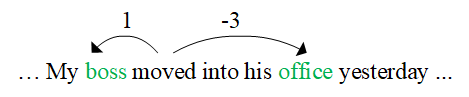
\includegraphics[]{postion.png}
  \caption{Example of position embeddings.}
  \label{PF}
\end{figure}

The final representation $\mathbf{x}_i$ of each word $w_{i}$ is the concatenation of the word embedding and two position embeddings as follows:
\begin{equation}
  \mathbf{x}_i = \mathbf{w}_i \oplus p_{i}^{e_{1}}\oplus p_{i}^{e_{2}}
\end{equation}
The symbol $\oplus$ represents concatenation operator.
Then the input representation part transforms an instance into a matrix $\mathbf{X}\in \mathbb{R}^{m \times d}$, where $m$ is the sentence length and $d = d_{w}+2d_{p}$.
The matrix $\mathbf{X}$ is subsequently fed into the convolutional part.

\subsubsection*{Piecewise CNN}
After representing all words in the sentence $x$ into their input embeddings, we employ PCNN as our feature extractor.
PCNN uses a piecewise max-pooling layer to capture sentence structure information. 
A sentence is divided into three segments by two entity words, then max-pooling is executed on each segment respectively.
Inheriting the settings from Zeng et al.\cite{zeng2015distant}, we apply tanh as activation function.
We denote convolution kernel channels by $d_{s}$,and the output of PCNN by $\mathbf{f}_x \in \mathbb{R}^{3d_{s}}$.
Figure ~\ref{Architecture PCNN} shows PCNN architecture for input representation.

\begin{figure}[h]
  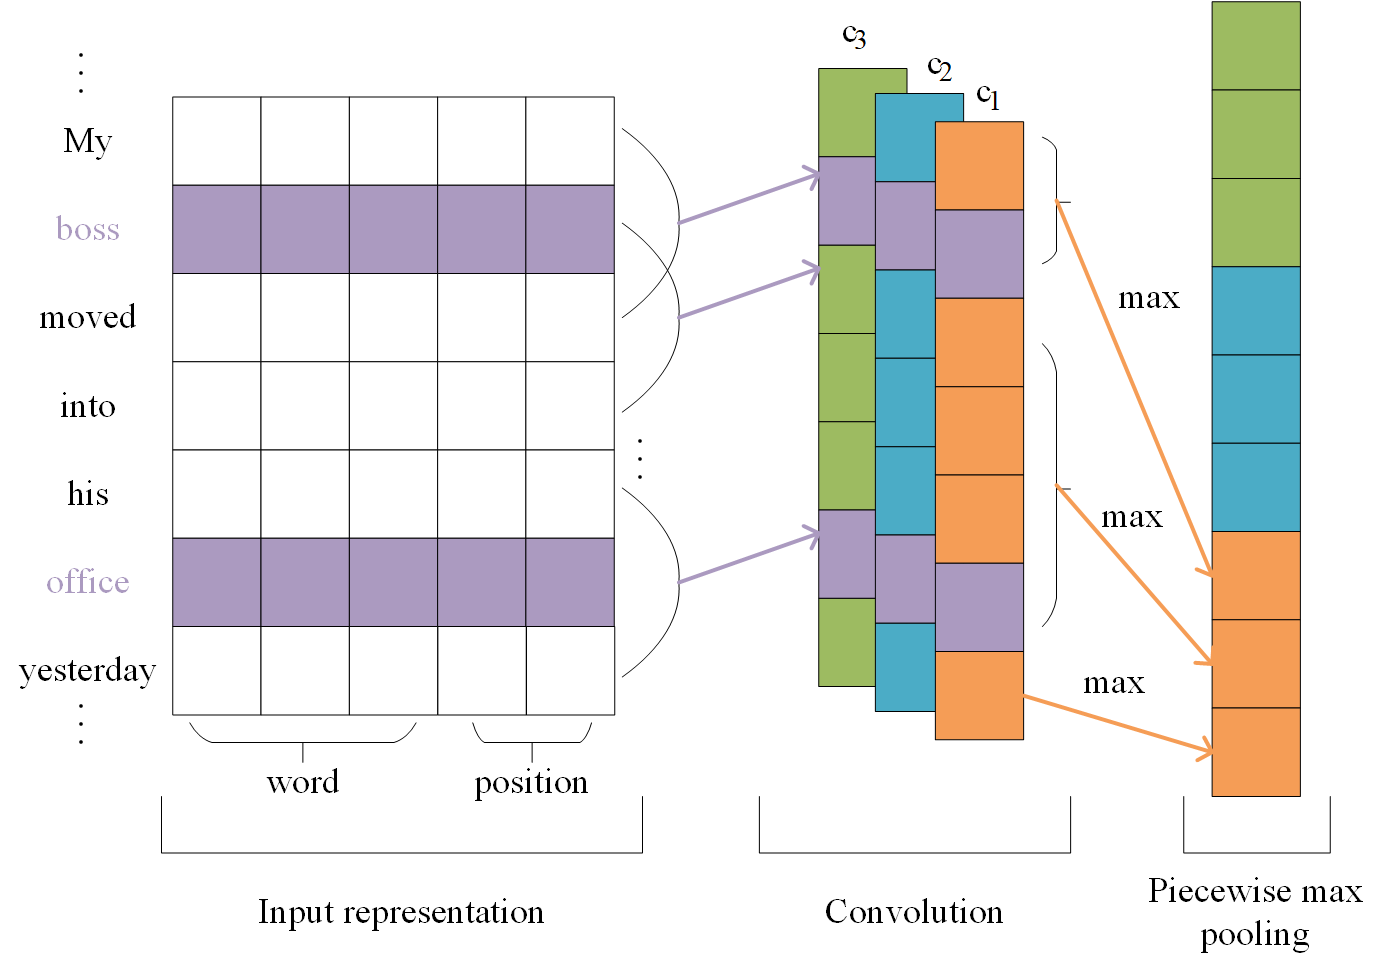
\includegraphics[height=6cm]{PCNN.png}
  \caption{PCNN Module is used to extract features.}
  \label{Architecture PCNN}
\end{figure}

\textbf{Convolution.}
Convolution is an operation between a vector of weights,
$\mathbf{w}$, and a vector of inputs that is treated as a sequence $\mathbf{X}$.
The weights matrix $\mathbf{w}$ is regarded as the filter for the convolution. 
In the example shown in Figure ~\ref{Architecture PCNN},
we assume that the length of the filter is $w (w=3) $;
thus, $\mathbf{w} \in \mathbb{R}^{w \times d}$.
We consider \textbf{S} to be a sequence $\left \{\mathbf{x}_1, \mathbf{x}_2, .., \mathbf{x}_m  \right \}$,
where $x_i \in \mathbb{R}^d$.
In general,
let $x_{i:j}$ refer to the concatenation of $x_i$ to $x_j$.
The convolution operation involves taking the dot product of \textbf{w} with each w-gram in the sequence $\mathbf{X}$ to obtain another sequence $\mathbf{c} \in \mathbb{R}^{m+w-1}$:
\begin{equation}
  c_j = \mathbf{w}\mathbf{x}_{j-w+1:j} 
\end{equation}
where the index j ranges from 1 to $m+w-1$.
Outof-range input values $\mathbf{x}_i$, where $i < 1$ or $i > m$, 
are taken to zero.
The ability to capture different features typically requires the use of multiple filters (or feature maps) in the convolution.
Under the assumption that we use $n$ filters $( W = \left\{{ w_1, w_2, ..., w_n} \right\})$,
the convolution operation can be expressed as follows:
\begin{equation}
  c_{ij} = \mathbf{w}_i\mathbf{x}_{i-w+1:j} \quad 1 \leq i \leq n
\end{equation}
The convolution result is a matrix $\mathbf{C} = \left\{\mathbf{c}_1, \mathbf{c}_2, ..., \mathbf{c}_n\right\} \in \mathbb{R}^{n\times(m+w-1)}$.
Figure \ref{Architecture PCNN} shows an example in which we use 3 different filters in the convolution procedure.

\textbf{Piecewise Max Pooling.}
The size of the convolution output matrix $\mathbf{C} \in \mathbb{R}^{n\times(m+w-1)} $ depends on the number of tokens $m$ in the sentence that is fed into the network.
An input sentence can be divided into three segments based on the two selected entities. 
Then, we propose a piecewise max pooling procedure that returns the maximum value in each segment instead of a single maximum value. 
As shown in Figure 3, the output of each convolutional filter $\mathbf{c}_i$ is divided into three segments $\left\{\mathbf{c}_{i1},\mathbf{c}_{i2},\mathbf{c}_{i3}\right\}$
by boss and office.
The piecewise max pooling procedure can be expressed as follows:
\begin{equation}
  p_{ij} = max(\mathbf{c}_{ij}) \quad 1 \leq i \leq n,1 \leq j \leq 3
\end{equation}
For the output of each convolutional filter,
we can obtain a 3-dimensional vector $\mathbf{p}_i = \left\{p_{i1},p_{i2},p_{i3}\right\}$.
We then concatenate all vectors $\mathbf{p}_{1:n}$.
Finally,
the piecewise max pooling procedure outputs a vector:
\begin{equation}
  \mathbf{f}_x = tanh(\mathbf{p}_{1:n})
\end{equation}

\subsection{Adversarial Training}
\label{sect:ad}
Although our strategy discovers a large amount of instances, it introduces a lot of noise.
Therefore, we can use there noisy data for adversarial training.
The purpose of discriminator is to identify relation types for each instance in datasets.
When given a noisy instance, the discriminator is also expected to resist noise and explicitly classify it into the correct label.  
Unlike the generator applied in computer vision field \cite{im2016generating} that generates a new image from the input noise, our generator aims to select instances from ND to confuse the discriminator as much as possible.
So we denote the generator as selector.

As shown in Figure 1, we exploit a supervised dataset SD and a noisy dataset ND.
Each instance $x \in SD$ express its relation type $r$ explicitly.
On the contrary, each instance $x \in ND$ is assumed to be unreliable.
However, there is a certain probability that it is labeled correctly.
Therefore, we train the selector to select the instances that are most likely to be labeled correctly to fool the discriminator by conditional probability $P\left(r\mid x\right), x \in ND$.
Meanwhile, we design the discriminator as a multi-class classifier, which aims at maximizing the conditional probability $P\left(r\mid x\right), x\in SD$ and $1-P\left(r\mid x\right), x\in ND$.
Based on the notion of adversarial training, we define the training process as an adversarial min-max game as follows: 
\begin{equation}
\begin{aligned}
  \underset{\theta_{D}}{max }\mathbb{E}_{x\sim P_{SD}}\left [ log\left ( P\left ( r\mid x \right ) \right ) \right ]+ \\
  \mathbb{E}_{x\sim P_{ND}}\left [log\left ( 1-P\left ( r\mid x \right ) \right ) \right ], \\
  \underset{\theta_{S}}{max }\mathbb{E}_{x\sim P_{ND}}\left [ log\left ( P\left ( r\mid x \right ) \right ) \right ],
\end{aligned}
\end{equation}
where $\theta_{D}$ and $\theta_{S}$ are the parameters of discriminator and selector respectively.
$P_{SD}$ is the supervised data distribution and selector samples adversarial examples from ND according to the probability distribution $P_{ND}$.
After our adversarial training process, we obtain a robust discriminator that can boost resistance to noise and better categorize relations and a selector that can select those informative instances with a higher probability compared with those noisy ones.

\textbf{Discriminator}

Given a sentence $x$ and its relation type $r \in \varepsilon$, the discriminator is responsible for predicting the relation type of this sentence.
After representing the sentence $x$ with its embedding $\mathbf{f}_x$, the feature vector $\mathbf{f}_x$ is fed into a softmax classifier, the discriminator calculates the probability of each relation type as follows, 
\begin{equation}
  \mathbf{o} = \mathbf{W}_1\mathbf{f}_x+\mathbf{b}
\end{equation}
$\mathbf{W}_1 \in \mathbb{R}^{n_{1}\times 3d_s}$ is the transformation matrix, where $n_{1}$ is equal to the number of relation types.
To obtain the conditional probability $P\left(r\mid x\right)$, we utilize the one-hot embedding of relation type:
\begin{equation}
  P\left(r\mid x\right) = \frac{\exp\left ( \mathbf{r}\cdot\mathbf{o} \right ) }{\sum_{k=1}^{n_{1}}\exp\left ( o_{k} \right )}
\end{equation}
where $\mathbf{r}$ is the one-hot embedding of the relation type $r\in \varepsilon$.
The optimized discriminator will assign high scores to those instances from SD and conversely distrust those instances in ND.
Hence, the objective of the discriminator can be formulated as minimizing the following loss function:
\begin{equation}
\begin{aligned}
  L_{D} = -\sum_{x\in SD}\frac{1}{\left | SD \right |}log\left ( P(r\mid x) \right ) -\\
  \sum_{x\in ND}P_{ND}(x)log(1-P(r\mid x))
\end{aligned}
\end{equation}
where $P_{ND}(x)$ is a probability computed by selector.The update of discriminator contains the parameters of encoder and $\theta_{D}$.

\textbf{Selector}

The selector is used to select the most confusing instances from ND to confuse the discriminator.
After representing the sentence $x$ with its embedding $\mathbf{f_{x}}$, the selector computes confusing probability $P_{ND}(x)$ for all instances in ND as follows, 
\begin{equation}
  P_{ND}(x) = \frac{1}{1+\exp(-(\mathbf{W}_2\mathbf{f}_x + b))}
\end{equation} 
where $\mathbf{W}_2 \in \mathbb{R}^{1\times3d_{s}}$ is the transformation matrix. 
In order to confuse the discriminator, the objective of the selector is to maximize the probabilities $P_{ND}$.
Hence, we can formalize the loss function to optimize the selector as follows, 
\begin{equation}
  L_{S} = -\sum_{x\in ND}P_{ND}(x)\log(P(r\mid x))
\end{equation}
where $P(r\mid x)$ is computed by the discriminator.
What needs to be explained is that, because the selector and the discriminator share one sentence encoder, we freeze the parameters of the encoder when optimizing the selector.
\subsection{Implementation Details}
As the common setting for GANs \cite{qin2018dsgan, Wang2019AdversarialTF}, we propose a pre-train process.
The discriminator and the selector share one sentence encoder, therefore we just pre-train the discriminator with SD.
In the implementation, we employ dropout \cite{JMLR:v15:srivastava14a} on the output layer of the encoder.
We call our approach as PCNN-AD. 

\subsection{Extend Dataset with Selector}
\label{sect:extend}
We construct the noisy dataset based on our discovery strategy with the entity pairs in the supervised data as heuristic seed.
For example, the entity pair ``\texttt{suicide}'' and ``\texttt{death}'' in the instance `` \texttt{suicide} is one of the leading causes of \texttt{death} among pre adolescents and teens ,  and victims of bullying are at an increased risk for committing suicide'' expresses the relation ``\texttt{Cause-Effect}'', then all instances in unlabeled data containing the entity pair ``\texttt{suicide}'' and ``\texttt{death}'' will be automatically labeled the relation ``\texttt{Cause-Effect}''.
Different from the distant supervision, our discovery strategy is restrictive, which can discover specific relation type to deal with the imbalance problem of the original dataset.
The details is shown in Section ~\ref{dataset}.
After our adversarial training process, we obtain a selector that can select the most confusing instances from noisy dataset meanwhile those instances are most likely to be labeled correctly. 
All instances from ND selected by the selector and regarded as being labeled correctly by the discriminator will be adjusted from ND to SD.
Thus, we obtain a extension of SD.

\section{Experiments}
Our experiments are intended to demonstrate that our method can obtain a large amount of data for supervised relation extraction and alleviate the noisy labeling problem.
To this end, we first introduce the dataset and evaluation metrics used.
Next, we show the detailed experimental settings, then compare the performance of our model to those several traditional methods.
Finally, we evaluate the effects of our selector and discriminator.

\subsection{Datasets and Evaluation}
\label{dataset}
To evaluate the performance of our model,
we conduct experiments on the \textbf{SemEval-2010 Task 8} dataset\cite{hendrickx2009semeval}.
The dataset consists of 8, 000 training and 2, 717 test sentences,
and each sentence is annotated with a relation between two given entities.
All instances are annotated with 9 directed relations types and an artificial class Other. 
Nine directed relations are respectively \textit{Cause-Effect, Instrument-Agency, Product-Producer, ContentContainer, Entity-Origin, Entity-Destination, ComponentWhole, Member-Collection, and Message-Topic}.
We take direction into consideration except \textit{Other} and the total number of relation types is 19. 
We construct a noisy dataset from the New York Times corpus with discovery strategy and use our adversarial training strategy to filter out the noisy instances to build a new dataset.
For balance, we discover 8000 instances as noisy data.
Figure ~\ref{Data distribution} shows the proportion of each relation type.
We followed the official task setting,  and report the official macro-averaged F1-score (Macro-F1) on the 9 relation types(excluding Other).
\begin{figure}[h]
  \centering
  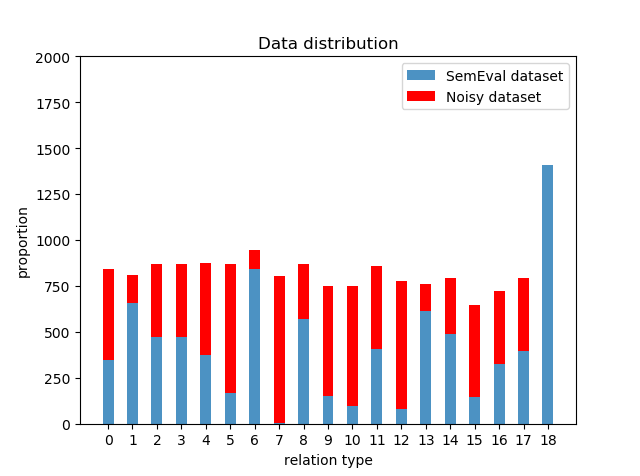
\includegraphics[width=8cm, height=6cm]{Datadistribution.png}
  \caption{Data distribution.Considering direction, We use two numbers to represent 
  each relation type respectively.}
  \label{Data distribution}
\end{figure}

\subsection{Experimental Settings}
\label{subsect:hyper}
For PCNN encoder, we follow the settings used in paper\cite{zeng2015distant} for fair comparisions,
we use the pre-trained word embeddings Glove \cite{pennington2014glove} as the initial word embeddings.
For adversarial training, we use a grid search to determine the optimal parameters and select learing rate $\lambda_{1}$ for S among $\left \{0.1, 0.01, 0.001, 0.005  \right \}$ and $\lambda_{2}$ for D among $\left \{0.1, 0.01, 0.001 \right \}$.  
Table ~\ref{parameters} shows the main parameters used in the experiments.
\begin{table}
\caption{\label{parameters} Hyperparameter settings}
  \centering
  \begin{tabular}{lrl}
  \hline \textbf{Hyperparameter} & \textbf{Value}\\ \hline
  Window size & 3\\
  Feature maps & 230\\
  Word embedding & 50\\
  Position embedding & 5\\
  Max sequence length & 128\\
  Training epochs & 5.0\\
  Learning rate of S, D & 0.005, 0.01\\
  Dropout rate & 0.5\\
  \hline
  \end{tabular}
  
  \end{table}

\subsection{Comparison with other Methods}
\subsubsection*{Overall Evaluation Results}
Results of various neural models are demonstrated in table ~\ref{F1}.
We compare our model with various neural baselines, including SVM, RNN, CNN, Attention CNN and Attention BiLSTM.
Table ~\ref{F1} reports the results.
We can see that our model significantly beats all the baseline models.
The MACRO F1 value of PCNN-AD is 87.61, which is much better than the previous methods.
\begin{table}[h]
\caption{\label{F1} Comparison with results in the literature.}
  \centering
  \begin{tabular}{|l|l|}
  \hline
  \multicolumn{1}{|c|}{Method} & F1   \\ \hline
  SVM (Rink and Harabagiu, 2010) \cite{Rink} & 82.2 \\ \hline
  RNN (Socher et al., 2012) \cite{socher2012semantic} & 77.6 \\ \hline
  CNN (Zeng et al., 2014) \cite{zeng2014relation} & 82.7 \\ \hline
  CR-CNN (Santos et al., 2015) \cite{dos-santos-etal-2015-classifying} & 84.1 \\ \hline
  Attention CNN (Shen and Huang, 2016) \cite{shen-huang-2016-attention} & 85.9 \\ \hline
  Attention BiLSTM (Lee et al., 2019) \cite{DBLP:journals/corr/abs-1901-08163} & 85.2 \\ \hline
  PCNN-AD                      & 87.61 \\ \hline
  \end{tabular}
  
  \end{table}

In order to avoid the impact of the augmented data on the results, we add noisy data and filtered data to the original dataset respectively, and conduct experiments with CNN and PCNN model.
Table ~\ref{results} shows the results on three datasets.
We can see that adding noisy data to the original data has no effect on the model even reduces its accuracy, and models trained on the filtered dataset perform better.
That demonstrates that our selector can select valid training instance which labeled correctly and improve the accuracy of models.
\begin{table}[h]
    \caption{\label{results} The F1 results(excluding Other) on different datasets of previous models. }
  \centering
  \begin{tabular}{lcl}
  \hline \textbf{Method} &\textbf{dataset} &\textbf{F1}\\ \hline
  CNN & \multicolumn{1}{c}{\begin{tabular}[c]{@{}c@{}}SemEval\\+Noisy \\ +Filtered \end{tabular}} & \begin{tabular}[c]{@{}l@{}}82.7\\ 81.8\\ 83.3\end{tabular}\\ \hline
  PCNN & \multicolumn{1}{c}{\begin{tabular}[c]{@{}c@{}}SemEval\\+Noisy \\ +Filtered \end{tabular}} & \begin{tabular}[c]{@{}l@{}}83.1\\ 82.9\\ 84.5\end{tabular}\\ \hline
  \end{tabular}
  
  \end{table}

\subsection{Case Study}
To demonstrate that our approach does select effective noisy instances, we give an example in Table ~\ref{case study}.
All hyperparameter are the same as those described in Section ~\ref{subsect:hyper}.

The instance in the ``SemEval'' row is a typical instance of the \textit{Entity-Destination} relation,
the instances in the  ``Discovered'' row are sampled from the noisy dataset constructed by our discovery strategy,
and the instance in the ``Extended'' row is selected from the noisy dataset by our selector.
Compared to most of discovered instances which are totally unrelated,
the instances selected by selector always express this relation.
This demonstrates that our methods can filter out noisy instances and accomplish utilizing large amount of unlabeled data to enrich labeled data. 
\begin{table}[h]
\caption{\label{case study} The example of extended data.}
\begin{center}
  \begin{tabular}{lc}
  \hline \textbf{dataset}&\textbf{Entity-Destination(e1, e2)} \\ \hline
  SemEval & several cats ran into\\
  &rob's garage\\ \hline
  Discovered& some cats left the garage\\ 
  & those cats are in the garage\\ 
  & cats walk into the garage\\ \hline
  Extended & cats walk into the garage\\ \hline
  \end{tabular}
\end{center}
  \end{table}

\section{Conclusion and Future Work}
In this paper, we take advantage of adversarial training and propose an effective method for supervised RE.
To be specific, we design a selector and discriminator framework with PCNN. 
The selector selects higher quality adversarial examples, which allow the discriminator model to learn better, as well as automatically construct a large dataset.
The experiments show that the adversarial training framework brought significant improvements to relation extraction.
In the future,  we plan to explore the following directions:
(1) We will propose our adversarial training method based on advanced sentence encoder.
(2) We will develop a large-scale and clean dataset for RE based on our method,  which will benefit further research in this field.

\section*{Acknowledgments}
The research reported in this paper was supported in part by the Nationnal Natural Science Foundation of China under the grant No.U1936104.

\bibliographystyle{IEEEtran}
\bibliography{./nrepapers}

\end{document}
